\documentclass[compress, aspectratio=54]{beamer}
%\documentclass[notes=show]{beamer}
%\documentclass[xcolor=dvipsnames]{beamer}
\usepackage[export]{adjustbox}
\usepackage{sidecap}
\usepackage{subfig}
\usepackage{amssymb}
\usepackage{latexsym}
\usepackage{amsfonts}
\usepackage{amsmath}
\usepackage[absolute,overlay]{textpos}
\usepackage[english]{babel}
\usepackage[latin1]{inputenc}
\usepackage{subfig}
%\usepackage{times}
\usepackage[T1]{fontenc}
\usepackage{tabularx}
\newcolumntype{Y}{>{\small\raggedright\arraybackslash}X}
\usepackage{graphicx}
\usepackage{bigstrut}
\usepackage{bbm}
\usepackage{mathrsfs}
\usepackage{epsfig}
\usepackage{array}
%\usepackage{natbib}
\usepackage{hyperref}
\usepackage{caption}
\usepackage{xcolor}

\mode<presentation> {
%\usetheme[left,width=1.7cm]{Berkeley}
%\usetheme{default}
\usetheme{Boadilla}
  \usecolortheme[RGB={103,102,204}]{structure}
%\usecolortheme{dove}
  \useoutertheme{infolines}
  \setbeamercovered{transparent}
 }

%\usepackage[utf8]{inputenc}

% Default fixed font does not support bold face
\DeclareFixedFont{\ttb}{T1}{txtt}{bx}{n}{12} % for bold
\DeclareFixedFont{\ttm}{T1}{txtt}{m}{n}{12}  % for normal

% Custom colors
\usepackage{color}
\definecolor{deepblue}{rgb}{0,0,0.5}
\definecolor{deepred}{rgb}{0.6,0,0}
\definecolor{deepgreen}{rgb}{0,0.5,0}

\usepackage{listings}

% Python style for highlighting
\newcommand\pythonstyle{\lstset{
language=Python,
basicstyle=\ttm,
otherkeywords={self},             % Add keywords here
keywordstyle=\ttb\color{deepblue},
emph={MyClass,__init__},          % Custom highlighting
emphstyle=\ttb\color{deepred},    % Custom highlighting style
stringstyle=\color{deepgreen},
frame=tb,                         % Any extra options here
showstringspaces=false            % 
}}


% Python environment
\lstnewenvironment{python}[1][]
{
\pythonstyle
\lstset{#1}
}
{}

% Python for external files
\newcommand\pythonexternal[2][]{{
\pythonstyle
\lstinputlisting[#1]{#2}}}

% Python for inline
\newcommand\pythoninline[1]{{\pythonstyle\lstinline!#1!}}
%\renewcommand{\familydefault}{cmss}
%\renewcommand{\mathrm}{\mathsf}
%\renewcommand{\textrm}{\textsf}
\usefonttheme{serif}
\newcommand{\X}{{\mathbf{X}}}
\newcommand{\x}{{\mathbf{x}}}
\newcommand{\E}{\mathsf{E}}
\newcommand{\V}{\mathsf{Var}}

\DeclareGraphicsExtensions{.jpg,.pdf,.mps,.png}

\setbeamercolor{bibliography entry title}{fg=black}
\setbeamercolor{bibliography entry author}{fg=black}
\setbeamercolor{subsection in toc}{fg=structure}
\setbeamercolor{palette primary}{bg=structure, fg=white}
%\setbeamercolor{palette secondary}{bg=structure, fg=black}
%\setbeamercolor{palette tertiary}{bg=structure, fg=black}
\setbeamercolor{caption name}{fg=black} \setbeamersize{text margin
left=.8cm} \setbeamersize{text margin right=1cm}
\hypersetup{linkbordercolor={1 0 0}} \setbeamertemplate{navigation
symbols}{} \setbeamertemplate{headline}[default]

\setbeamertemplate{enumerate items}[default]

\newcounter{transfct}
\newcounter{begbs}
\newcounter{endbs}


\title[Intro to Text Analysis]{Introduction to Text Analysis}

\author[Arieda Mu\c co]{Arieda Mu\c co}
\institute[CEU]{Central European University}
\date{}
\AtBeginSection[] {
  \begin{frame}<handout:0>
    \frametitle{TOC}
    \tableofcontents[currentsection]
  \end{frame}
}


\AtBeginSection[] {
  \begin{frame}<handout:0>
    \frametitle{TOC}
    \tableofcontents[currentsection]
  \end{frame}
}


\pgfdeclareimage[height=.7cm]{logo}{rgs2}
\logo{\pgfuseimage{logo}}
\begin{document}
\captionsetup[subfigure]{labelformat=empty}

\frame{\titlepage}

\begin{frame}
\frametitle{"Usual" Data}
\begin{itemize}
\item A spreadsheet with continuous and discrete variables (ready for analysis!?), fixed number of columns
\begin{itemize}
\item Real data is messy and almost never ready for analysis
\end{itemize}

\item Data can come from images, audio, video, text and there is no (fixed) number of columns

\end{itemize}
\end{frame}
%----------------------------------------------------------------------------%

\begin{frame}
\frametitle{Common data}
\begin{figure}

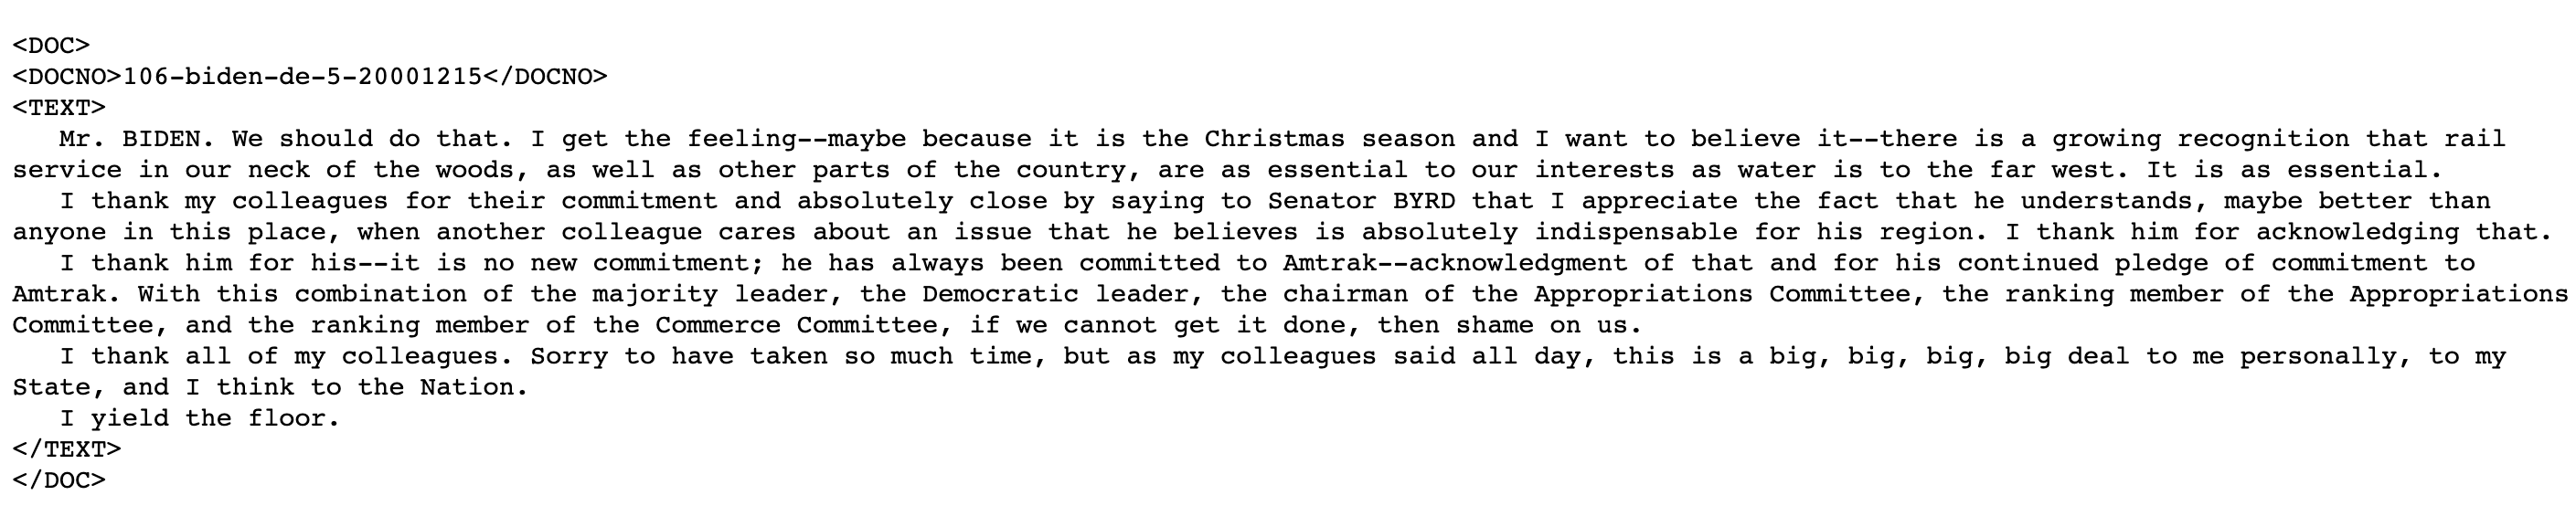
\includegraphics[width=1\linewidth ]{Figures/biden}
\end{figure}
\begin{figure}

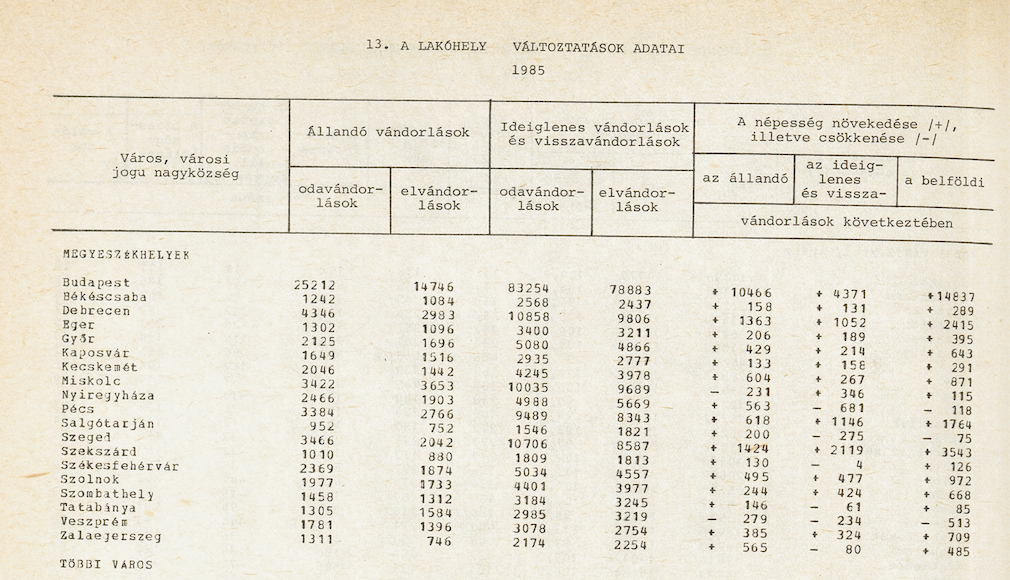
\includegraphics[width=0.8\linewidth ]{Figures/ksh-data}
\end{figure}
\end{frame}


\begin{frame}
\frametitle{Also common data}
\begin{figure}

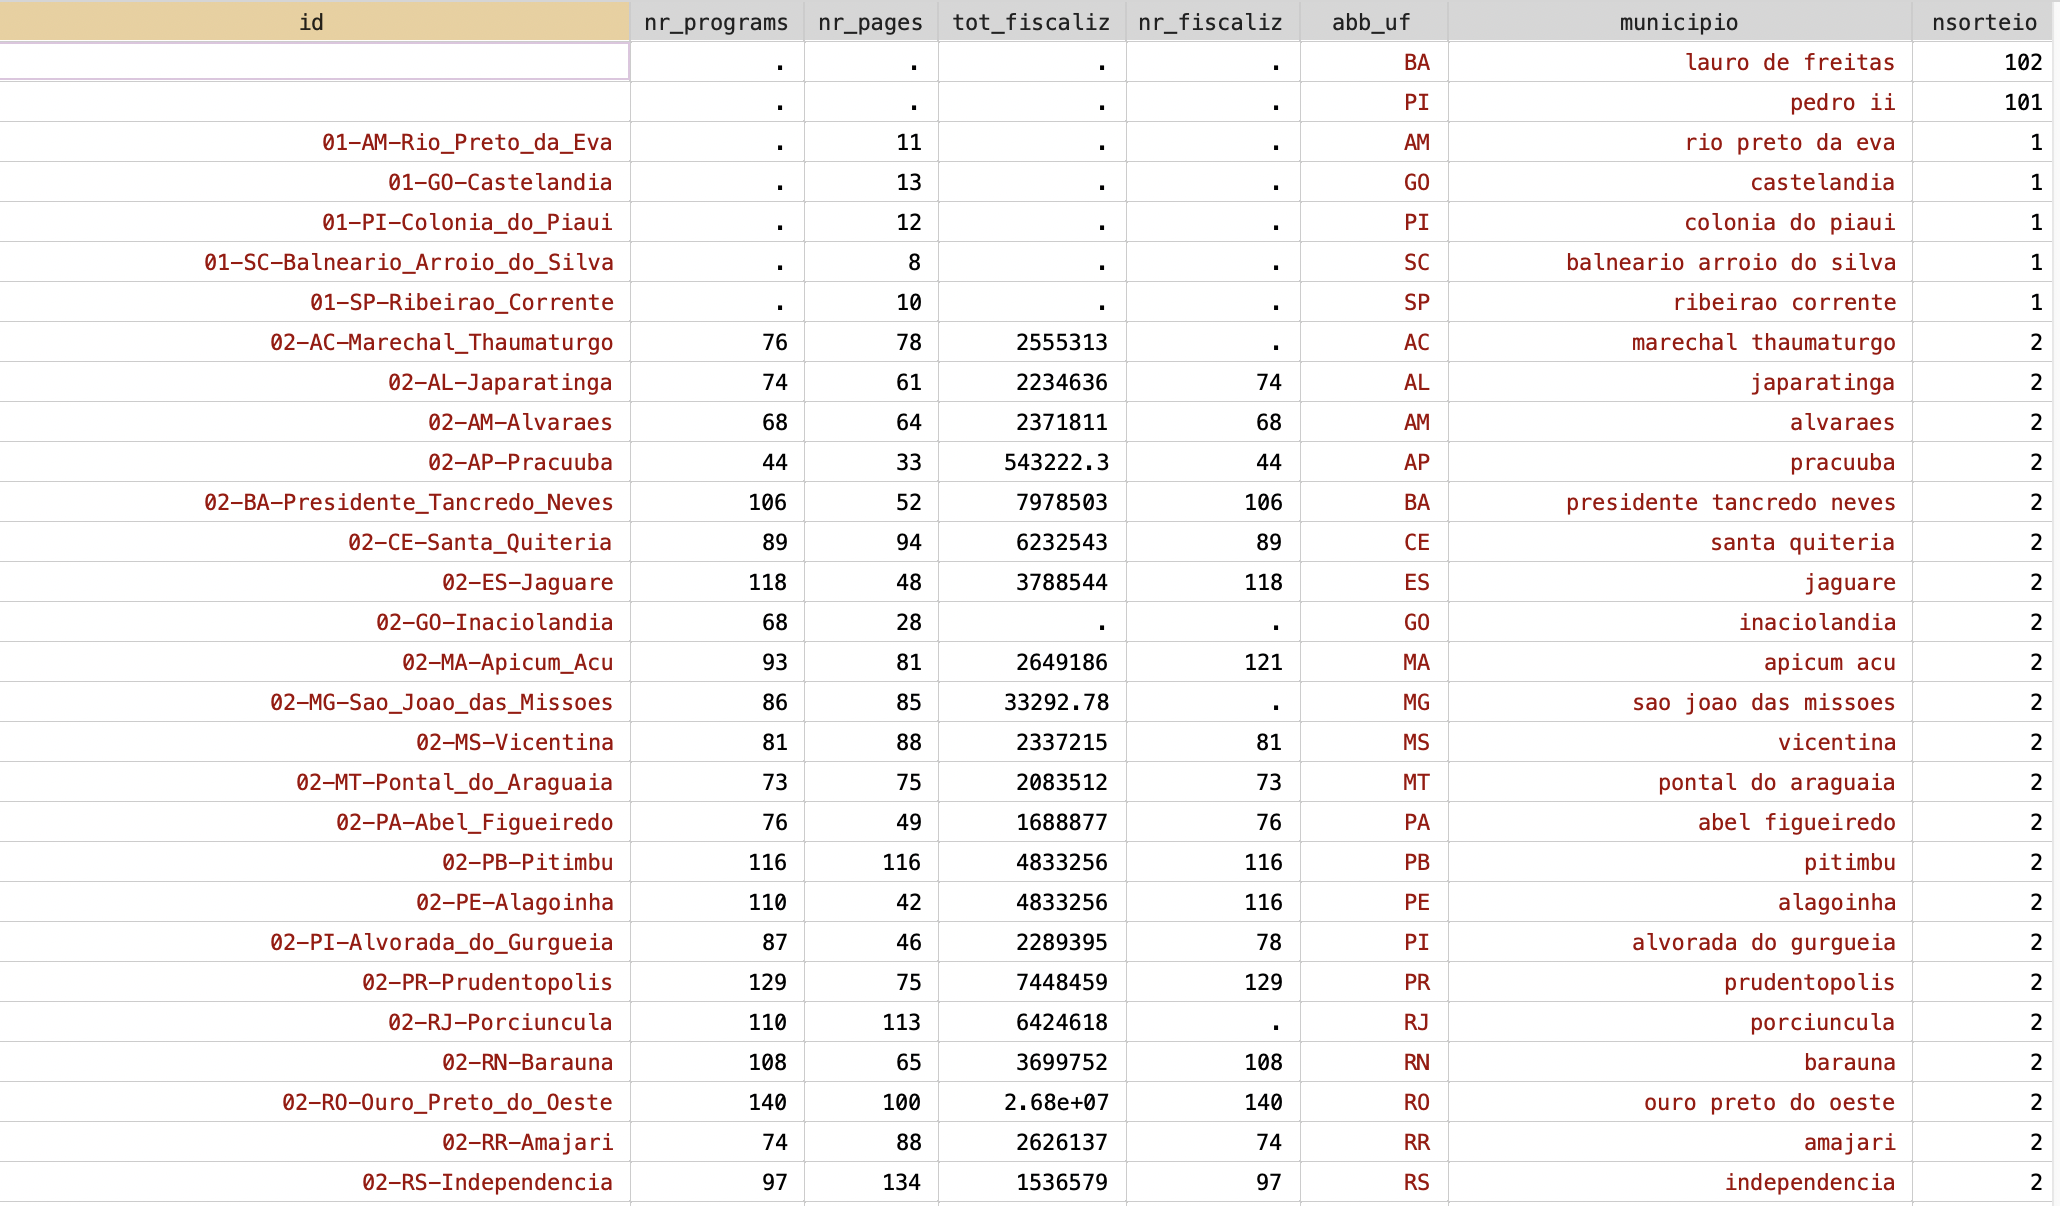
\includegraphics[width=0.9\linewidth ]{Figures/text-data2}
\end{figure}
\end{frame}
%----------------------------------------------------------------------------%

\begin{frame}
\frametitle{Text as Data}
\begin{itemize}
\item Classify an email message as either a
legitimate email or spam
\item Learn about the opinion of a politician on the topic of
immigration

\item The content of the text will certainly contain important information for the task
\item Text data is usually represented as concatenation of characters. In
any of the examples just given, the length of the text data will vary
\item This feature is clearly very different from the numeric features, and we will need to process the data before we can
apply algorithms to it

\end{itemize}
\end{frame}
%----------------------------------------------------------------------------%

\begin{frame}
\frametitle{Preprocessing}
\begin{itemize}
\item Make it useful for our purposes
\item Simplify and lower dimensionality

\end{itemize}
\end{frame}
%----------------------------------------------------------------------------%



%----------------------------------------------------------------------------%

\begin{frame}
\frametitle{Document - Term}
\begin{figure}

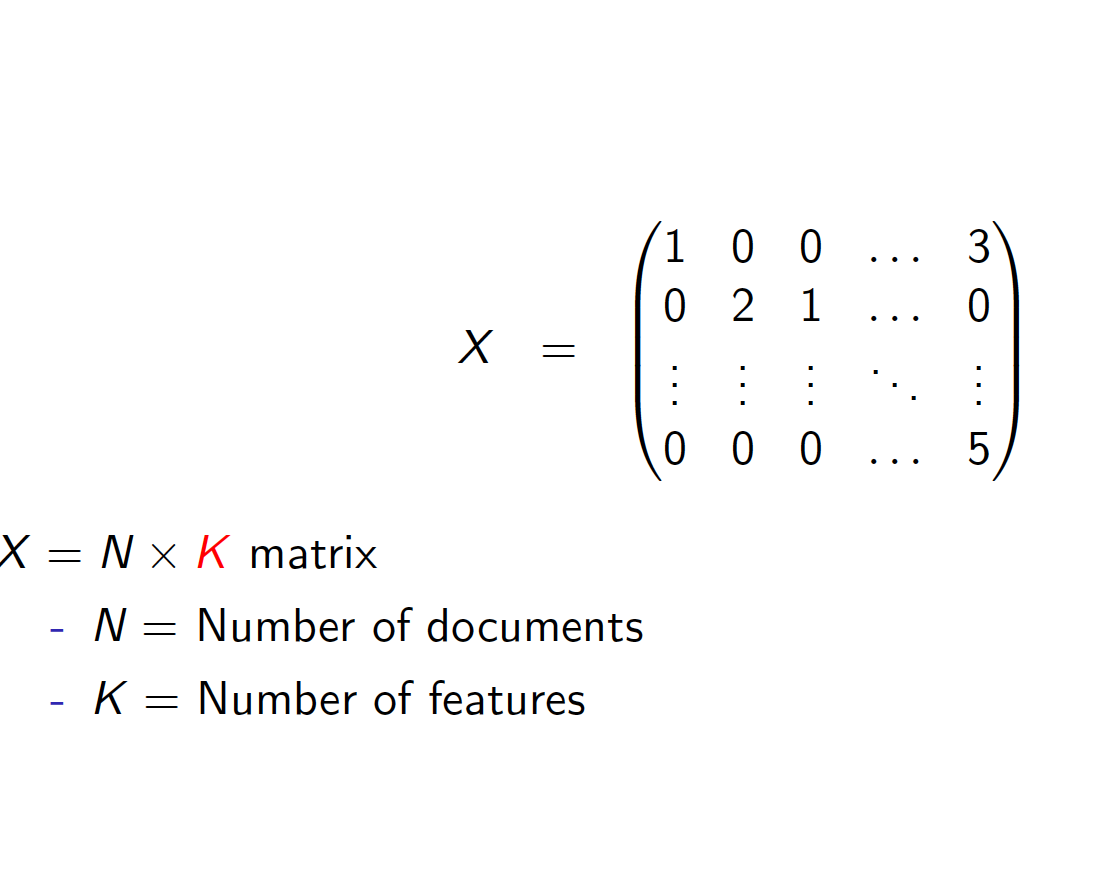
\includegraphics[width=0.5\linewidth ]{Figures/document_term.png}
\end{figure}

\end{frame}


%----------------------------------------------------------------------------%

\begin{frame}
\frametitle{Preprocessing for Quantitative Text Analysis}
Recipe for preprocessing: retain useful information
\begin{itemize}
\item Remove capitalization, punctuation
\item Discard stop words
\item Discard Word Order (Bag of Words Assumption)
\item Create Equivalence Class: Stem, Lemmatize, or synonym
\item Discard less useful features (depends on application)
\item Other reduction, specialization


\end{itemize}
Output: Count vector, each element counts occurrence of stems
\end{frame}
%----------------------------------------------------------------------------%

%----------------------------------------------------------------------------%

\begin{frame}
\frametitle{Stop Words}
Stop Words: English Language place holding words
\begin{itemize}
\item the, it, if, a, able, at, be, because...
\item Add ``noise" to documents (without conveying much information)
\item Discard stop words: focus on substantive words
\item \textbf{Caution}: Exercise caution when discarding stop words. You may need to customize your stop word list.
\end{itemize}
\end{frame}
%----------------------------------------------------------------------------%

%----------------------------------------------------------------------------%

\begin{frame}
\frametitle{Creating an Equivalence Class of Words}
Reduce dimensionality further (create equivalence class between words)
\begin{itemize}
\item Words used to refer to same basic concept. 
\begin{itemize}
\item family, families, familial $\rightarrow$ famili
\end{itemize}

\item Stemming/Lemmatizing algorithms: Many-to-one mapping from
words to stem/lemma
\end{itemize}
\end{frame}
%----------------------------------------------------------------------------%

%----------------------------------------------------------------------------%

\begin{frame}
\frametitle{Stemming vs Lemmatization}
\begin{itemize}
\item Stemming algorithm: 
\begin{itemize}
\item Consists of chopping off end of word
\item Porter stemmer, Lancaster stemmer, Snowball stemmer
\end{itemize}

\item Lemmatizing algorithm:
\begin{itemize}
\item Condition on part of speech (noun, verb, etc)
\item Verify result is a word
\end{itemize}

\end{itemize}
\end{frame}
%----------------------------------------------------------------------------%
%----------------------------------------------------------------------------%

\begin{frame}
\frametitle{ Stemming vs Lemmatization}
\begin{itemize}
\item Stemming algorithm: 
\begin{itemize}
\item Word representations may not have any
meaning
\item Takes less time
\item Use stemming when meaning of words is
not important for analysis. Example: Spam
detection.

\end{itemize}

\item Lemmatizing algorithm:
\begin{itemize}
\item Word representations have meaning
\item Takes more time than Stemming
\item Use lemmatization when meaning of
words is important for analysis. Example:
question answering application.
\end{itemize}

\end{itemize}
\end{frame}
%----------------------------------------------------------------------------%

%----------------------------------------------------------------------------%

\begin{frame}
\frametitle{Stemming -vs- Lemmatization}
\begin{figure}

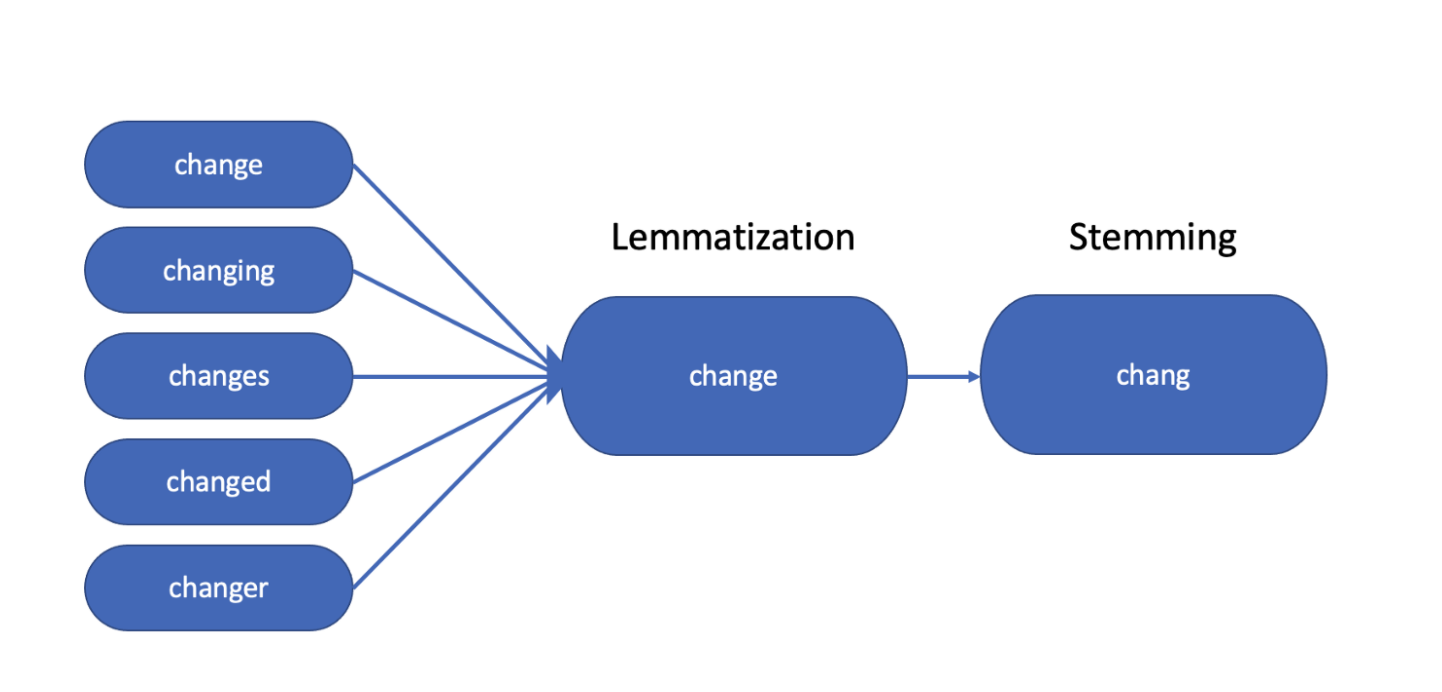
\includegraphics[width=0.8\linewidth ]{Figures/stemming-vs-lemmatization.png}
\end{figure}

\end{frame}


%----------------------------------------------------------------------------%

\begin{frame}
\frametitle{Additional read}
Stemming and Lemmatization -- Stanford NLP\\
\url{https://nlp.stanford.edu/IR-book/html/htmledition/stemming-and-lemmatization-1.html}
\end{frame}
%----------------------------------------------------------------------------%
%----------------------------------------------------------------------------%

\begin{frame}
\frametitle{}
Preprocessing reduces dimensionality where it causes problems for
inference (stopwords, stemming) and sometimes increases
dimensionality when it makes our inferences better (bigram, ngrams)
\end{frame}



\begin{frame}
\frametitle{A Complete Example}
Assume our document contains the following sentence: ``I love cats and dogs" 
\begin{itemize}

\item \textbf{Bag of Words (BoW)}:  We retain each word discarding their order 

\item \textbf{ngram}: An analyst may want to combine words into a single
term that can be analyzed. If you think ``love'' and ``cats'' should be together we form a bigram
\end{itemize}

\end{frame}
%----------------------------------------------------------------------------%

\begin{frame}
\frametitle{Bag of words }
[I], [love], [cats], [and], [dogs] 

\begin{itemize}
\item Each word is represented as a token
\end{itemize}
\end{frame}

%----------------------------------------------------------------------------%

\begin{frame}
\frametitle{Remove stopwords}
[love], [cats],  [dogs] 
\begin{itemize}

\item \textbf{Remove Stopwords}: Removing terms that do not convey important information. Different schools of thought
\end{itemize}

\end{frame}
%----------------------------------------------------------------------------%



\begin{frame}
\frametitle{Stemming -Lemmatization}
[love], [cat],  [dog] 
\begin{itemize}

\item \textbf{Stemming}: Takes the ends of conjugated verbs or plural nouns, leaving just the stem.
\end{itemize}
\end{frame}
%----------------------------------------------------------------------------%

%----------------------------------------------------------------------------%

\begin{frame}
\frametitle{Assume we have a second document}
Document 2: ``Cats are adorable.''\\
\end{frame}
%----------------------------------------------------------------------------%




\begin{frame}
\frametitle{Document Term Matrix}

Original Documents:

Document 1: ``I love cats and dogs.''

Document 2: ``Cats are adorable.''

Document-Term Matrix:

\[
\begin{bmatrix}
 & \text{{cat}} & \text{{dog}} & \text{{love}} & \text{{adorable}} & \text{{are}} \\
\text{{Document 1}} & 1 & 1 & 1 & 0 & 0 \\
\text{{Document 2}} & 1 & 0 & 0 & 1 & 1 \\
\end{bmatrix}
\]
\end{frame}



%----------------------------------------------------------------------------%

%----------------------------------------------------------------------------%

\begin{frame}
\frametitle{All steps together}

\begin{enumerate}
\item Remove capitalization and punctuation
\item Discard word order (Bag of Words)
\item Remove stop words
\item Applying Stemming Algorithm
\item Create count vector or one hot encoded vector
\end{enumerate}
\end{frame}


%----------------------------------------------------------------------------%


\begin{frame}
\frametitle{Vectorization a simple example}
You have 2 documents:
\begin{enumerate}
\item  Blue House
\item Red House
\end{enumerate}
 Our corpus will consist of all the words in the documents namely: Red, Blue, House. The vector representation in the  ``Bag of Words" approach: 

\begin{itemize}

\item "Blue House" -> (red, blue, house) -> (0, 1, 1)
\item "Red House" -> (red, blue, house) -> (1, 0, 1)
\end{itemize}

Once we have vector representation, we can do analysis. Algorithms can handle numbers (vectors)
\end{frame}
%----------------------------------------------------------------------------%


%----------------------------------------------------------------------------%

\begin{frame}
\frametitle{Cosine Similarity}
Cosine similarity is a measure of similarity between two non-zero vectors of an inner product space.  The cosine similarity is particularly used in positive space, text data,  where the outcome is neatly bounded in $[0,1]$

\[
sim(A, B)=cos(\Theta)= \frac{A \cdot B}{\| A \| \| B \|}
\]
\begin{figure}

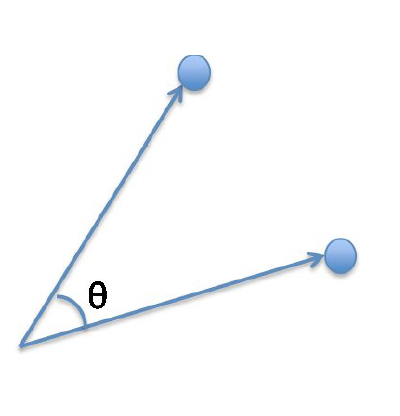
\includegraphics[width=0.2\linewidth ]{Figures/cosine_sim.png}
\end{figure}
\end{frame}
%----------------------------------------------------------------------------%


%----------------------------------------------------------------------------%

\begin{frame}
\frametitle{Term Frequency and Inverse Document Frequency}
\begin{itemize}

\item Improve on Bag of Words by adjusting word
counts based on their frequency in corpus (the group of
all the documents)

\item Use Term Frequency - Inverse Document Frequency (TF-IDF)
\end{itemize}


\end{frame}

%----------------------------------------------------------------------------%

\begin{frame}
\frametitle{TF-IDF}
TF-IDF term x in document y
\[
TF_{x,y} \times log (\frac{N}{DF_x} )
\]
\begin{itemize}
\item $ TF_{x,y} =$ frequency of x in y
\item $DF_x =$ number of documents containing x
\item $N$ total number of documents
\end{itemize}

\end{frame}
%----------------------------------------------------------------------------%


%----------------------------------------------------------------------------%
%----------------------------------------------------------------------------%

\begin{frame}
\frametitle{TF-IDF}
\begin{itemize}

\item[TF]  Term- Frequency is the raw frequency of a word normalized by the number of words in the document
\item [IDF] Inverse Document Frequency is the number of documents normalized by the number of documents that contain the term. For terms that are present in every document, this will lead to an IDF value of zero (that is, log(1)). For this reason, one of the possible normalizations for IDF is 1+log(N/$DF_x$)

\end{itemize}

\end{frame}
%----------------------------------------------------------------------------%


%----------------------------------------------------------------------------%

%----------------------------------------------------------------------------%

\begin{frame}
\frametitle{TF-IDF}
The intuition behind TF-IDF is that words which are too frequent or too rare are not representative
\begin{figure}

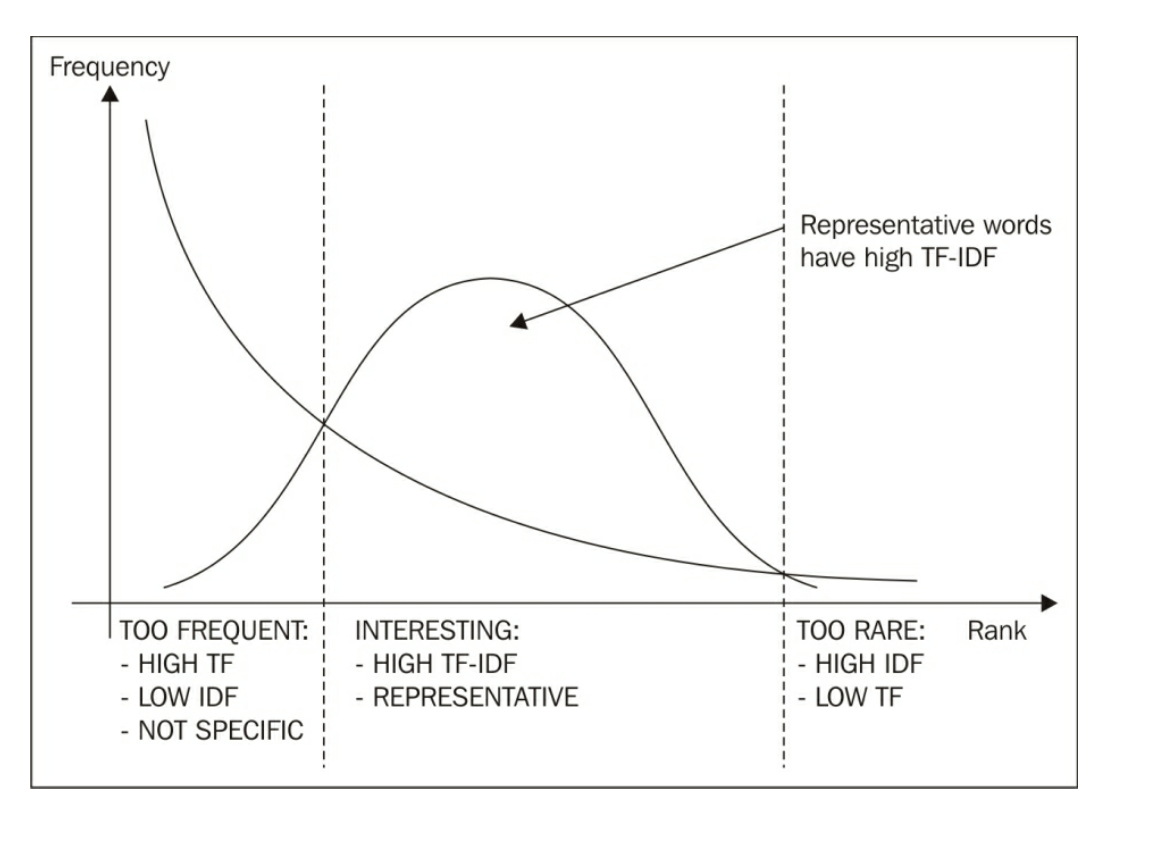
\includegraphics[width=0.65\linewidth ]{Figures/tf-idf.png}
\end{figure}
\end{frame}
%----------------------------------------------------------------------------%



%----------------------------------------------------------------------------%

\begin{frame}
\frametitle{How can this work?}

\begin{itemize}
\item Speech may contain sarcasm:
\begin{itemize}

\item The Star Wars prequels were amazing because everyone
loves a good discussion about trade policy
\end{itemize}

\item Subtle Negation
\begin{itemize}

\item They have not succeeded, and will never succeed, in
breaking the will of this valiant people
\end{itemize}
\item Order Dependence
\begin{itemize}
\item Peace, no more war
\item War, no more peace
\end{itemize}
\end{itemize}
\end{frame}


%----------------------------------------------------------------------------%


%----------------------------------------------------------------------------%

\begin{frame}
\frametitle{How Could This Possibly Work?}

\begin{enumerate}
\item It might not: Validation is critical (task specific)

\item Central Tendency in Text: Words often imply what a text is about
war, civil, union or tone consecrate, dead, died, lives.
Likely to be used repeatedly: create a theme for an article

\item Human supervision: Inject human judgement (coders): helps methods
identify subtle relationships between words and outcomes of interest

\end{enumerate}
It is easier to capture some things than others
\end{frame}






\end{document}


